%% Revised SISC manuscript, 11 October 2026.
%% Build with latexmk -pdf -interaction=nonstopmode -halt-on-error paper.tex.
\documentclass[review,hidelinks,letterpaper]{siamart251216}
\usepackage[numbers,sort&compress]{natbib}
\usepackage{amssymb,amsfonts,graphicx,booktabs,enumitem,microtype}
\newsiamremark{remark}{Remark}
\newsiamremark{example}{Example}
\newcommand{\creflastconjunction}{, and~}
\setlist{nosep,leftmargin=1.6em}
\setlength{\emergencystretch}{2em}
\AtBeginEnvironment{thebibliography}{\interlinepenalty=10000}
\headers{Error Covariance in Block Floating Point}{Y. Xiong}
\title{Exact Error Covariances for Block Floating Point Reductions}
\author{Yongkang Xiong\thanks{College of Changkong, Nanjing University of
Aeronautics and Astronautics, 29 Jiangjun Avenue, Nanjing 211106, China
(\email{nuaapanda@outlook.com}).}}
\hypersetup{pdftitle={Exact Error Covariances for Block Floating Point Reductions},
 pdfauthor={Yongkang Xiong}}
\begin{document}
\maketitle
\begin{abstract}
Selecting a shared scale from a block maximum couples the quantization errors.
We derive exact finite-block error moments from one-dimensional truncated
distributions, including continuous laws and atoms. For identically distributed
independent inputs, the conditional pair covariance is nonpositive;
variation of the conditional mean supplies a competing positive contribution.
The resulting covariance gives the variance and mean-square error of weighted
reductions. Dropping the conditional pair correction while retaining the
conditional moments overestimates sum-variance inflation by at most one.
The formulas extend to independent heterogeneous inputs and, by conditioning,
to correlated inputs with latent factors. An exponential-input theorem shows
that variance inflation can diverge along a dyadic subsequence despite
vanishing pair correlation and finite moments of every order.
Rational enumeration, high-precision integration, and Monte Carlo validate
the moment calculations. Two-dimensional elliptic experiments connect the
moments to solution energy error, spatial block layout, and precision allocation
at a fixed storage budget. At seven bits per source value, spatial precision
placement reduces measured RMS error by 22.4\% relative to uniform placement;
a uniform-noise model selects a codec with 4.1\% higher error than the best
tested candidate. Correlated-source experiments retain cross-block dependence
through the latent-factor mixture. Bit-packing audits and conjugate-gradient
solves verify the format and predicted input-conversion errors. An independent train/validation
experiment tests allocation after estimating the source law from data.
\end{abstract}
\begin{keywords}
block floating point, quantization, rounding error, covariance,
weighted reduction, stochastic rounding
\end{keywords}
\begin{AMS}
65G50, 65F35, 60G70
\end{AMS}
\section{Introduction}\label{sec:intro}
Block floating point represents a vector by integer coefficients and a common
power-of-two scale. The scale is usually selected from the block maximum,
so it depends on the same data that are subsequently rounded. This choice
couples the rounding errors. In a sum or a matrix--vector product, even a
small covariance between two coordinates can matter because it contributes
once for every coordinate pair. Predicting the variance of an individual
error is therefore insufficient for predicting the error of a reduction.

Classical statistical quantization models approximate residuals by centered
uniform noise \cite{widrow1996,widrow2008}. Block floating point roundoff
has a long history \cite{kalliojarvi1996}, and statistical noise models
continue to inform accelerator design \cite{song2018,lian2019}.
Microscaling formats add a contemporary motivation \cite{ocpmx2023}.
The shared-scale dependence is also
recognized: Rohani and Fakhraie \cite{rohani2006} discuss correlations in
dynamically rescaled structures, and Soloveychik et al.
\cite{soloveychik2022} use maximum order statistics to derive inner-product
error bounds and study block-size selection for Gaussian data. The latter
model approximates nonmaximum residuals by uniform noise. Fox and Lindstrom
\cite{fox2026zfp} analyze systematic bias in the ZFP compression pipeline.
These studies leave a finite-block question: how can one compute the error
covariance of a maximum-selected quantizer directly from the input law?

We derive such a calculation from one-dimensional truncated moments.
For independent, identically distributed inputs, conditioning on a binade
of the maximum excludes the event that every coordinate lies below its
lower endpoint. This exclusion gives an explicit nonpositive conditional
covariance. Variation of the conditional error mean across binades supplies
a competing nonnegative contribution. Their sum determines whether a
reduction is inflated or attenuated. The calculation also extends to
independent inputs with different distributions, for which the conditional
pair correction can have either sign. Conditioning on latent factors then
provides moments for correlated inputs and covariances between blocks.

The covariance matrix gives exact variance and mean-square error formulas
for deterministic weighted reductions. It also provides a useful
approximation guarantee: retaining the conditional moments while dropping
the negative pair correction overestimates the sum's variance inflation
factor by at most one. Thus the approximation becomes relatively accurate
when inflation is large, while the full formula resolves small inflation
and deflation. The complete covariance matrix supplies the moments needed
for propagation through a linear operator.

The large-block limit reveals a separate obstruction. Bounded support with
a nondegenerate limiting error gives unit inflation. With unbounded support,
the pair correlation tends to zero, yet the number of pairs can amplify it.
An exponential-input counterexample proves that inflation diverges along a
dyadic subsequence even though every input moment is finite. A decreasing
pair correlation therefore cannot justify an independent-error model for
large reductions.

Our numerical study checks the formulas by exact rational enumeration,
high-precision integration, and independently sampled blocks. Weighted
reductions expose the role of cancellation and bias; elliptic solves connect
the covariance to solution accuracy, block layout, and a fixed storage
budget. A train/validation experiment tests the same allocation after the
source law is estimated rather than supplied. Symmetric inputs and independently randomized stochastic rounding
provide controls through their zero pair covariance
\cite{connolly2021,croci2022}. These results complement probabilistic
analyses of arithmetic rounding \cite{higham2019,higham2020,hallman2023},
mixed-precision kernels \cite{fasi2023}, fixed-quantizer inner-product
distortion \cite{ang2026quant}, and state-conditioned reduction trees
\cite{sao2026trees}. The contribution here is the dependence created when
the input quantizer selects its own common scale.

\section{Exact finite-block analysis}\label{sec:exact}

Let $X_1,\ldots,X_n$ be independent copies of a real random variable $X$,
where $n\ge2$, $\mathbb E[X^2]<\infty$, and $L$ is a fixed nonnegative
integer. Set $M_n=\max_i|X_i|$. When $M_n>0$, define
\begin{equation}\label{eq:revision-format}
 K_n=\lfloor\log_2 M_n\rfloor,\qquad s_k=2^{k-L},\qquad
 h_k(x)=s_k\operatorname{RN}(x/s_k)-x,\qquad e_i=h_{K_n}(X_i),
\end{equation}
with round-to-nearest, ties-to-even on an unsaturated uniform integer grid.
The all-zero block has state $*$ and zero errors.
The analysis treats input conversion; weights and linear operators are fixed.
Independent heterogeneous laws and conditionally independent inputs are
introduced in Section~\ref{sec:nonidentical}. For a selected nonzero block,
$|X_i/s_{K_n}|<2^{L+1}$, so the rounded integer coefficient has magnitude
at most $2^{L+1}$. A signed integer of width $L+3$ therefore suffices,
including rounding to the positive endpoint. The experimental codecs use an
8-bit signed block exponent and count all coefficient and padding bits.

The error vector is exchangeable because its construction commutes with
permutations of the inputs. Write
\begin{equation}\label{eq:revision-statistics}
 \mu=\mathbb E[e_1],\quad v=\operatorname{Var}(e_1)>0,\quad
 \kappa=\operatorname{Cov}(e_1,e_2),\quad
 \mathcal I_n=\frac{\operatorname{Var}(\sum_i e_i)}{nv}
             =1+(n-1)\frac{\kappa}{v}.
\end{equation}
The positivity of $v$ is needed only for ratios; the moment identities below
also hold when $v=0$.

\subsection{A closed conditional covariance formula}

Use the strict distribution function
$G(t)=\mathbb P(|X|<t)$ for $t>0$. For an exponent $k$, put
\begin{equation}\label{eq:revision-truncations}
 \begin{gathered}
 a_k=2^k,\quad b_k=2^{k+1},\quad p_k=G(a_k),\quad q_k=G(b_k),\\
 P_k=q_k^n-p_k^n,\qquad
 T_{\ell,k}(t)=\mathbb E[h_k(X)^\ell\mathbf 1_{\{|X|<t\}}].
 \end{gathered}
\end{equation}
The use of strict inequalities assigns atoms at $a_k$ and $b_k$ to the
correct binades. The exponent states have total mass
$1-\mathbb P(X=0)^n$; the remaining mass $P_*=\mathbb P(X=0)^n$ belongs to $*$.

\begin{theorem}[Exact conditional moments and negative conditional covariance]
\label{thm:revision-exact}
For every $k$ with $P_k>0$, define
$m_k=\mathbb E[e_1\mid K_n=k]$,
$t_k=\mathbb E[e_1^2\mid K_n=k]$, and
$c_k=\operatorname{Cov}(e_1,e_2\mid K_n=k)$. Then
\begin{align}
 m_k&=\frac{q_k^{n-1}T_{1,k}(b_k)-p_k^{n-1}T_{1,k}(a_k)}{P_k},
       \label{eq:revision-moment1}\\
 t_k&=\frac{q_k^{n-1}T_{2,k}(b_k)-p_k^{n-1}T_{2,k}(a_k)}{P_k},
       \label{eq:revision-moment2}\\
 \mathbb E[e_1e_2\mid K_n=k]
   &=\frac{q_k^{n-2}T_{1,k}(b_k)^2-p_k^{n-2}T_{1,k}(a_k)^2}{P_k}.
       \label{eq:revision-pair}
\end{align}
If $p_k>0$, put
$u_k=T_{1,k}(a_k)/p_k$,
$z_k=T_{1,k}(b_k)/q_k$, and $r_k=(p_k/q_k)^n$. Then
\begin{equation}\label{eq:revision-negative}
 m_k=\frac{z_k-r_k u_k}{1-r_k},\qquad
 c_k=-\frac{r_k}{(1-r_k)^2}(z_k-u_k)^2\le0.
\end{equation}
Products associated with a zero-probability event in
\eqref{eq:revision-pair} are understood as zero, including when $n=2$.
If $p_k=0$, the formulas reduce to $m_k=z_k$ and $c_k=0$.
The same identities hold for any measurable deterministic scalar response
$h_k$ applied identically to each coordinate, with the required moments.
\end{theorem}

\begin{proof}
The event $\{K_n=k\}$ is the difference between the nested events
$\{M_n<b_k\}$ and $\{M_n<a_k\}$. Independence gives
\begin{align*}
 \mathbb E[h_k(X_1)\mathbf 1_{\{M_n<t\}}]
     &=G(t)^{n-1}T_{1,k}(t),\\
 \mathbb E[h_k(X_1)h_k(X_2)\mathbf 1_{\{M_n<t\}}]
     &=G(t)^{n-2}T_{1,k}(t)^2.
\end{align*}
Subtract the expressions at $t=a_k$ from those at $t=b_k$ and divide by
$P_k$. The second-moment identity follows in the same way. Substitution of
$T_{1,k}(a_k)=p_k u_k$ and $T_{1,k}(b_k)=q_k z_k$ yields
$\mathbb E[e_1e_2\mid K_n=k]=(z_k^2-r_k u_k^2)/(1-r_k)$.
Subtracting $m_k^2$ gives \eqref{eq:revision-negative}. If $p_k=0$,
conditioning only truncates each input at $b_k$, preserving independence.
\end{proof}

The sign in \eqref{eq:revision-negative} has a precise origin. Conditioning
on the exponent first restricts every input to $|X_i|<b_k$, then excludes
the event that all inputs satisfy $|X_i|<a_k$. The resulting selection
induces a nonpositive covariance between two copies of the same scalar
response. Consequently, conditional uncorrelatedness is an additional
restriction, not a consequence of sharing the exponent: when $p_k>0$, it
holds exactly if $u_k=z_k$.

For the state $*$, set $m_*=t_*=c_*=0$. Including this state in every sum,
the complete population quantities are
\begin{align}
 \mu&=\sum_k P_km_k,&
 v&=\sum_kP_kt_k-\mu^2,\label{eq:revision-global}\\
 B&=\operatorname{Var}(m_{K_n})
      =\sum_kP_k(m_k-\mu)^2,&
 C&=\sum_kP_kc_k\le0,\qquad \kappa=B+C.
 \label{eq:revision-decomposition}
\end{align}
The term $B$ describes variation of the conditional mean between exponent
states; $C$ is the negative correction within a state. Their sum can have
either sign.

\begin{corollary}[A certified bound for omitting the conditional covariance]
\label{cor:revision-bracket}
Let $A=\mathbb E[\operatorname{Var}(e_1\mid K_n)]$, so $v=A+B$. Then
\begin{equation}\label{eq:revision-bracket}
 \frac{nB}{v}\le\mathcal I_n
       \le1+(n-1)\frac{B}{v}\le n,
 \qquad
 0\le \left(1+(n-1)\frac{B}{v}\right)-\mathcal I_n\le\frac{A}{v}\le1.
\end{equation}
\end{corollary}

\begin{proof}
The law of total variance gives
$\operatorname{Var}(\sum_i e_i)
=\mathbb E[\operatorname{Var}(\sum_i e_i\mid K_n)]+n^2 B\ge n^2B$.
The upper bound follows from $C\le0$ in
$\mathcal I_n=1+(n-1)(B+C)/v$; subtracting the lower bound proves the
absolute-error estimate. Finally $B\le v$.
\end{proof}

Omitting $C$ therefore overestimates $\mathcal I_n$ by at most one. When
$\mathcal I_n>0$, its relative error is at most $1/\mathcal I_n$; the
absolute bound remains valid at the positive-semidefinite boundary
$\mathcal I_n=0$.

\subsection{Weighted reductions and rounding controls}

The covariance matrix has the form
\begin{equation}\label{eq:revision-spectrum}
 \Sigma=(v-\kappa)I+\kappa\mathbf 1\mathbf 1^T.
\end{equation}
Its eigenvalues are $v-\kappa$ in the $n-1$ directions orthogonal to
$\mathbf1$, and $v+(n-1)\kappa=v\mathcal I_n$ in the common direction.
Both are nonnegative, giving the usual bounds $0\le\mathcal I_n\le n$.
For deterministic weights $w\in\mathbb R^n$, the error in an exact reduction
of the quantized inputs is $E_w=\sum_iw_ie_i$. In particular,
\begin{equation}\label{eq:revision-weighted}
 \mathbb E[E_w]=\mu\mathbf1^Tw,\qquad
 \mathbb E[E_w^2]=(v-\kappa)\|w\|_2^2
                  +(\kappa+\mu^2)(\mathbf1^Tw)^2.
\end{equation}
This separates coherent bias from covariance. For an unweighted sum,
$\mathbb E[E_{\mathbf1}^2]=nv\mathcal I_n+n^2\mu^2$; an inflation factor
alone therefore does not measure its mean-square error. For $\mathbf1^Tw=0$,
the bias and the common-direction contribution vanish.

The effect of deleting $C$ depends on the weights. If $V_w$ denotes the
true centered variance and $\widetilde V_w$ is obtained by replacing
$\kappa=B+C$ by $B$ while retaining $v$, then
\begin{equation}\label{eq:revision-weighted-approximation}
 \widetilde V_w-V_w
 =-C\bigl((\mathbf1^Tw)^2-\|w\|_2^2\bigr),\qquad
 |\widetilde V_w-V_w|
 \le\frac{A}{n-1}
       \bigl|(\mathbf1^Tw)^2-\|w\|_2^2\bigr|
 \le A\|w\|_2^2.
\end{equation}
Indeed, Corollary~\ref{cor:revision-bracket} gives
$0\le-C\le A/(n-1)$, and Cauchy--Schwarz gives the last inequality.
The same difference applies to mean-square error because the retained bias
is unchanged. For weights summing to zero, deleting $C$ underestimates the
centered variance; for an unweighted sum it overestimates it.

\begin{proposition}[Symmetry and stochastic-rounding controls]
\label{prop:revision-controls}
For the quantizer in \eqref{eq:revision-format}, a distribution symmetric
about zero gives $m_k=c_k=0$ for every state, hence $\mu=\kappa=0$ and
$\mathcal I_n=1$ whenever $v>0$. For stochastic rounding with independent
rounding choices conditional on the full input block, $\mu=\kappa=0$ for
any input law, even without independence between the inputs. Its marginal
variance is
\begin{equation}\label{eq:revision-sr}
 v_{\rm SR}=\mathbb E[s_{K_n}^2\theta_1(1-\theta_1)],\qquad
 \theta_1=\operatorname{frac}(X_1/s_{K_n}),
\end{equation}
with the integrand zero in the all-zero state.
\end{proposition}

\begin{proof}
Oddness of round-to-nearest on symmetric truncation sets gives
$T_{1,k}(t)=0$, and Theorem~\ref{thm:revision-exact} proves the first claim.
Here stochastic rounding means ideal independent random bits conditional on
the complete input block; finite-bit implementations require a separate
randomness audit. Stochastic rounding has conditional mean zero and second moment
$s^2\theta_i(1-\theta_i)$ \cite{connolly2021,croci2022}.
Independent choices give zero conditional cross moments; taking expectations
proves \eqref{eq:revision-sr}.
\end{proof}

\begin{example}[Conditional exclusion can produce variance deflation]
\label{ex:revision-deflation}
Let $\mathbb P(X=13/10)=\mathbb P(X=41/20)=1/2$ and $L=2$.
An all-small block has step $1/4$ and every error is $-1/20$. Every other
block has step $1/2$; its small inputs have error $1/5$, and its large
inputs have error $-1/20$. Direct enumeration gives
\begin{equation}\label{eq:revision-deflation}
 \mathcal I_n=1-\frac{(n-1)4^{-n}}{1/4-4^{-n}}<1.
\end{equation}
At $n=2$, $v=3/256$, $\kappa=-1/256$, and $\mathcal I_2=2/3$.
The conditional-mean contribution is $B=1/768$, so omitting $C$ instead
predicts $10/9$. This reverses the qualitative conclusion.
\end{example}

\subsection{Independent inputs with different distributions}
\label{sec:nonidentical}

\begin{proposition}[Conditional moments for independent nonidentical inputs]
\label{prop:revision-nonidentical}
Let $X_1,\ldots,X_n$ be independent, each with a finite second moment, and
use the same maximum-selected grid as in \eqref{eq:revision-format}. At a
fixed exponent $k$ with $P_k>0$ (and hence $q_i>0$ for every $i$), write
$p_i=\mathbb P(|X_i|<a_k)$,
$q_i=\mathbb P(|X_i|<b_k)$, and
$P_k=\prod_iq_i-\prod_ip_i>0$. For $\ell\in\{1,2\}$ define
\[
 z_{\ell,i}=\mathbb E[h_k(X_i)^\ell\mid |X_i|<b_k],\qquad
 u_{\ell,i}=\mathbb E[h_k(X_i)^\ell\mid |X_i|<a_k]
 \quad\text{when }p_i>0.
\]
If every $p_i>0$, put $r=\prod_i(p_i/q_i)$. Then
\begin{align}
 \mathbb E[e_i^\ell\mid K_n=k]
   &=\frac{z_{\ell,i}-r u_{\ell,i}}{1-r},
       \label{eq:revision-nonidentical-marginal}\\
 \mathbb E[e_ie_j\mid K_n=k]
   &=\frac{z_{1,i}z_{1,j}-r u_{1,i}u_{1,j}}{1-r},\qquad i\ne j,
       \label{eq:revision-nonidentical-pair}\\
 \operatorname{Cov}(e_i,e_j\mid K_n=k)
   &=-\frac{r}{(1-r)^2}
       (z_{1,i}-u_{1,i})(z_{1,j}-u_{1,j}).
       \label{eq:revision-nonidentical-covariance}
\end{align}
If any $p_i=0$, the conditional inputs are independent under the upper
truncations: the marginal moments are $z_{\ell,i}$, the pair moments are
$z_{1,i}z_{1,j}$, and all conditional pair covariances are zero.
The all-zero state has probability $\prod_i\mathbb P(X_i=0)$ and zero
error moments.
\end{proposition}

\begin{proof}
On the upper rectangular event $\{M_n<b_k\}$, each marginal moment factors
as $\prod_iq_i$ times its normalized truncated moment; pair moments factor
as $\prod_iq_i$ times the product of the two truncated means. Subtract the
corresponding lower-event expressions and divide by $P_k$. Subtracting
the product of the conditional means yields
\eqref{eq:revision-nonidentical-covariance}. If any $p_i=0$, the lower
event has probability zero, leaving only independent upper truncations.
\end{proof}

The unconditional moments follow by mixing these states, including the
all-zero state. In particular, with
$m_{i,k}=\mathbb E[e_i\mid K_n=k]$ and
$c_{ij,k}=\operatorname{Cov}(e_i,e_j\mid K_n=k)$,
\[
 \operatorname{Cov}(e_i,e_j)
 =\operatorname{Cov}(m_{i,K_n},m_{j,K_n})+\sum_kP_kc_{ij,k}.
\]
The conditional covariance can have either sign because the two
truncated-mean differences need not agree in sign.

\begin{corollary}[Conditional mixtures]\label{cor:conditional-mixture}
Suppose the coordinates are independent conditional on a random variable
$Y$, and have finite unconditional second moments. Let $m(y)$ and $\Sigma(y)$
be the full error mean and covariance obtained from
Proposition~\ref{prop:revision-nonidentical} at $Y=y$. Then
\begin{equation}\label{eq:conditional-mixture}
 \mathbb E[e]=\mathbb E_Y[m(Y)],\qquad
 \operatorname{Cov}(e)=\mathbb E_Y[\Sigma(Y)]
                         +\operatorname{Cov}_Y(m(Y)).
\end{equation}
For several blocks, $\Sigma(y)$ is block diagonal; the second term includes
covariances between blocks.
\end{corollary}
\begin{proof}
Apply the conditional moment formulas for almost every $y$, followed by
total expectation and total covariance. Since $|e_i|\le|X_i|$,
the required moments are integrable.
\end{proof}

\section{Asymptotic behavior and an unbounded counterexample}\label{sec:revision-asymptotics}

Bounded support fixes the exponent eventually. Unbounded support forces
the grid to become arbitrarily coarse. The second mechanism removes
correlation between a fixed pair of errors, but does not guarantee that
the accumulated variance ratio tends to one.

\begin{proposition}[Bounded support and fixed-pair decorrelation]
\label{prop:revision-support}
The following statements hold at fixed $L$.
\begin{enumerate}
\item Suppose $|X|$ is bounded and
$k_* =\max\{k:\mathbb P(|X|\ge2^k)>0\}$ exists. Put
$p=\mathbb P(|X|<2^{k_*})<1$ and
$v_*=\operatorname{Var}(h_{k_*}(X))$. If $v_*>0$, then
\begin{equation}\label{eq:revision-bounded}
 v\longrightarrow v_*,\qquad |\kappa|=O(p^n),\qquad
 |\mathcal I_n-1|=O(np^n).
\end{equation}
If $p=0$, the exponent is fixed and $\mathcal I_n=1$ for every $n$.
\item Suppose $|X|$ has unbounded support and
$\sigma_X^2=\operatorname{Var}(X)>0$. Then
\begin{equation}\label{eq:revision-unbounded}
 \begin{gathered}
 e_i\longrightarrow-X_i\ \text{in }L^2\ \text{for each fixed }i,
 \qquad \mu\longrightarrow-\mathbb E[X],\\
 v\longrightarrow\sigma_X^2,\qquad
 \kappa\longrightarrow0,\qquad \frac{\mathcal I_n}{n}\longrightarrow0.
 \end{gathered}
\end{equation}
\end{enumerate}
\end{proposition}

\begin{proof}
For bounded support, $\mathbb P(K_n\ne k_*)=p^n$.
Couple $e_i$ to the fixed-step error $e_i^*=h_{k_*}(X_i)$ on the same
inputs. These errors coincide outside that event and are uniformly bounded.
Consequently, their first, second, and pair moments differ by $O(p^n)$.
The $e_i^*$ are independent, so $\kappa=O(p^n)$, and $v\to v_*>0$
gives \eqref{eq:revision-bounded}.

For unbounded support, realize all blocks as prefixes of an infinite i.i.d.
sequence. Almost surely $M_n\to\infty$, hence $s_{K_n}\to\infty$.
For each fixed $i$, eventually $|X_i|<s_{K_n}/2$, and
$\widehat X_i=0$. The grid includes zero, so its nearest point satisfies
$|e_i|\le|X_i|$ and $|\widehat X_i|\le2|X_i|$. Dominated convergence
gives $\widehat X_i\to0$ in $L^2$. The limits of $\mu$, $v$, and
$\kappa$ follow from this convergence and the independence of $X_1,X_2$.
Equation~\eqref{eq:revision-statistics} then gives $\mathcal I_n/n\to0$.
\end{proof}

The unbounded result cannot be strengthened to $\mathcal I_n\to1$ under
these assumptions. The factor $n-1$ in
\eqref{eq:revision-statistics} can amplify a covariance that tends to zero.
The following light-tailed example makes this obstruction explicit.

\begin{theorem}[Diverging inflation for exponential inputs]
\label{thm:revision-exponential}
Let $X\sim\operatorname{Exp}(1)$ and keep $L\ge0$ fixed. For
$a_j=2^j$ and $n_j=\lfloor\exp(a_j)\rfloor$, define
$\beta=2^{-L-2}$. Then
\begin{equation}\label{eq:revision-exp-asymptotic}
 \mathcal I_{n_j}\sim
 e^{-1}(1-e^{-1})\,2^{-2L-2}
          (\log n_j)^2n_j^{1-2\beta}
 \qquad (j\to\infty).
\end{equation}
In particular $\mathcal I_{n_j}\to\infty$, although
$\kappa_{n_j}\to0$ and $\mathcal I_{n_j}/n_j\to0$.
\end{theorem}

\begin{proof}
Throughout the proof, $a=a_j$ and $n=n_j$. The two exponent probabilities
are
\begin{align*}
 P_{j-1}&=(1-e^{-a})^n-(1-e^{-a/2})^n\longrightarrow e^{-1},\\
 P_j&=(1-e^{-2a})^n-(1-e^{-a})^n\longrightarrow1-e^{-1},
\end{align*}
because $ne^{-a}\to1$, $ne^{-a/2}\to\infty$, and $ne^{-2a}\to0$.
We first compute the conditional moments exactly, then control the
remaining exponent states to obtain the asymptotic equivalence.

For a fixed step $s$, the layer-cake formula for the nonnegative quantized
value gives
\begin{equation}\label{eq:revision-exp-response}
 H(s):=\mathbb E[s\operatorname{RN}(X/s)]
 =s\sum_{m=1}^{\infty}e^{-(m-1/2)s}
 =\frac{s e^{-s/2}}{1-e^{-s}},\qquad \mathbb E[h_s(X)]=H(s)-1.
\end{equation}
Here ties have probability zero. Away from ties, $h_s$ and $h_s^2$ are
periodic with period $s$. For a positive integer $m$ and either response
$\varphi=h_s$ or $h_s^2$, shifting the exponential tail gives
\[
 \mathbb E[\varphi(X)\mathbf1_{\{X\ge ms\}}]
   =e^{-ms}\mathbb E[\varphi(X)].
\]
Both binade endpoints are integer multiples of their step:
$a_k/s_k=2^L$, $b_k/s_k=2^{L+1}$. Consequently, truncation at either
endpoint preserves the normalized first and second response moments.
Theorem~\ref{thm:revision-exact} therefore gives, for every state,
$m_k=H(s_k)-1$ and $c_k=0$.
The second moment follows by integrating one period:
\[
 t_k=\frac{\int_0^{s_k/2}x^2e^{-x}\,dx
                +\int_{s_k/2}^{s_k}(s_k-x)^2e^{-x}\,dx}{1-e^{-s_k}}
       =2-2H(s_k).
\]
Thus, with $R=H(s_{K_n})$, the population moments have the closed form
\begin{equation}\label{eq:revision-exp-closed}
 \mu=\mathbb E[R]-1,\qquad v=1-(\mathbb E[R])^2,\qquad
 B=\operatorname{Var}(R),\qquad C=0.
\end{equation}

For state $j-1$, the step is $s_-=a/2^{L+1}$; the step in state $j$ is
$s_+=2s_-$. Put $H_-=H(s_-)$ and $H_+=H(s_+)$. By
\eqref{eq:revision-exp-response},
$H_-\sim2^{-L-1}a e^{-\beta a}$ and $H_+/H_-\to0$.
Also $H(s)=s/(2\sinh(s/2))$ is decreasing and satisfies $0<H(s)\le1$;
the explicit hyperbolic form gives $H'(s)<0$ and $H_+/H_-\to0$.
The derivative is negative for $s>0$, which also shows $H_+/H_-$ tends to zero.
The total probability of all lower states is
\[
 \delta_n=\mathbb P(K_n\le j-2)
       =(1-e^{-a/2})^n\le \exp(-ne^{-a/2})
       =\exp(-\sqrt n(1+o(1))).
\]
It follows that $\delta_n=o(H_-^2)$. In every upper state $k\ge j$,
$R\le H_+=o(H_-)$. These bounds control all omitted states: the lower
states contribute at most $\delta_n$ to either the first or the second
moment of $R$, and the upper states contribute at most $H_+$ and $H_+^2$,
respectively. Therefore
\[
 \mathbb E[R]=P_{j-1}H_-+o(H_-),\qquad
 \mathbb E[R^2]=P_{j-1}H_-^2+o(H_-^2),
\]
and hence
$B\sim e^{-1}(1-e^{-1})H_-^2$.
Equation~\eqref{eq:revision-exp-closed} gives $v\to1$ and
$\mathcal I_n=1+(n-1)B/v$. Since $1-2\beta>0$,
the latter expression is asymptotic to $nB$.
Finally $a/\log n\to1$ and $e^{-\beta a}\sim n^{-\beta}$, proving
\eqref{eq:revision-exp-asymptotic}.
\end{proof}

For $L=2$ the exponent in this asymptotic law is $7/8$. Thus a finite second
moment guarantees fixed-pair decorrelation but allows the inflation of a
block sum to grow without bound. The position of the block maximum relative
to powers of two matters even for an exponential tail.

\section{Computing the moments and designing the experiments}\label{sec:methods}
\subsection{A deterministic evaluator}
The statistical moment formulas are exact; their implementation evaluates
the required input integrals numerically. For a density $f$ and rounding
cell $J_{d,k}=[(d-1/2)s_k,(d+1/2)s_k)$, the continuous contribution is
\begin{equation}\label{eq:cell-integration}
 T_{\ell,k}(t)=\sum_d\int_{J_{d,k}\cap(-t,t)}
                         (d s_k-x)^\ell f(x)\,dx.
\end{equation}
Atoms contribute their probabilities times $h_k(x)^\ell$, with ties to
even. Expanding the integrand uses cell probabilities and the first two
truncated input moments. Since $t/s_k\le2^{L+1}$ at both binade endpoints,
each exponent requires $O(2^L)$ cells, independently of $n$.
For heterogeneous inputs, these integrals are evaluated coordinatewise.
The exponential identity \eqref{eq:revision-exp-closed} supplies a separate
closed-form check.

We form $G(t)^n$ from survival probabilities and logarithms, and use
\texttt{expm1} differences for nearby log probabilities.
Equation~\eqref{eq:revision-negative} evaluates the conditional covariance
stably; centered sums across exponent states evaluate $B$. The evaluator
records omitted exponent probability and numerical stability diagnostics.
The large-block exponential calculation uses higher precision to resolve
survival probabilities below binary64 resolution.

We compare four predictions. The \emph{finite-block prediction} uses
\eqref{eq:revision-global}--\eqref{eq:revision-decomposition}.
The \emph{conditional-mean upper prediction} retains $m_k,t_k,v$ and sets
$C=0$, as in Corollary~\ref{cor:revision-bracket}.
The \emph{unconditioned-response approximation} mixes moments of $h_k(X)$
under the original input law with $P_k$ and assumes conditional
independence. The \emph{uniform-noise prediction} uses
$\mu=\kappa=0$ and $v=\mathbb E[s_{K_n}^2]/12$.

For an iid law, the evaluator visits the retained exponent states and
integrates $O(2^L)$ rounding cells per state, so its scalar work is
$O(K2^L)$ for $K$ retained states and does not grow with the block length
$n$. For a heterogeneous block of size $b$, the corresponding work is
$O(K(b2^L+b^2))$ including covariance assembly; storage is $O(b^2)$.
This is the cost of the population evaluator, separate from Monte Carlo
sampling and from the linear solve used in the application experiments.

In the tables, ``Exact'' denotes numerical evaluation of the exact moment
identities. The heterogeneous and latent evaluators retain exponents
$-40\le k\le35$ and skip states of probability below $10^{-25}$.
They record omitted-probability and residual-energy bounds separately from
integration convergence checks. Numerical truncation bounds are therefore
part of the population prediction, rather than evidence supplied by its
Monte Carlo interval.
The application codecs use an 8-bit signed exponent and reject out-of-range
states; all retained source vectors and all population states lie inside that
range, so no saturation or exponent clipping is included in the reported
errors.

\subsection{Independent verification}
An independent rational oracle enumerates $25{,}600$ blocks in $96$
configurations: six finite-support laws,
$n\in\{2,3,4,6\}$, and $L\in\{0,1,2,4\}$.
It checks the conditional moments, covariance eigenvalues, weighted MSE,
and certified bracket, including atoms, zero blocks, dyadic endpoints,
and ties to even. A second oracle enumerates $480$ blocks in $32$
heterogeneous-input configurations and checks
Proposition~\ref{prop:revision-nonidentical}, including both conditional
covariance signs. Rational Green-matrix calculations verify linear
propagation against direct gradient energy in one and two dimensions.
Independent lognormal evaluators use analytical cell moments at $60$ and
$90$ decimal digits to check the homogeneous and heterogeneous moment
calculations. An $80$-digit Pareto cell integrator agrees with all eight
binary64 inflation factors to relative error below $8.1\times10^{-10}$.

\subsection{Sampling and measurement}
The main-grid and weighted experiments use independent blocks, master seed
$20261010$, and labeled child random streams. Population predictions are
computed from the input law. For each sampled block we retain
$S_b=\sum_i e_{b,i}$, $Q_b=\sum_i e_{b,i}^2$, exponent state, and squared
step, with $s_*=0$. For $B_{\rm MC}$ blocks,
\begin{equation}\label{eq:mc-estimator}
 \widehat\mu=\frac{\sum_b S_b}{nB_{\rm MC}},\quad
 \widehat v=\frac{\sum_b Q_b}{nB_{\rm MC}}-\widehat\mu^2,\quad
 \widehat{\mathcal I}_n=
   \frac{\operatorname{sampleVar}_b(S_b)}{n\widehat v}.
\end{equation}
The numerator has denominator $B_{\rm MC}-1$. Confidence intervals are
nominal $95\%$ percentile intervals from $200$ bootstrap resamples of whole
blocks. We use ``contains'' below to report whether a displayed interval
contains the population prediction; this is an empirical interval check,
not a repeated-sampling coverage theorem. Application-specific streams,
sample counts, and vector-bootstrap protocols are given with their
experiments.

The main grid uses $\mathcal N(0,1)$, $\exp(Z)$, $|Z|$, $\max(Z,0)$
for $Z\sim\mathcal N(0,1)$, $\operatorname{Exp}(1)$, and Pareto$(4)$
with $\mathbb P(X>x)=x^{-4}$ for $x\ge1$.
Combining $n\in\{32,128,512,4096\}$ with $L\in\{2,4\}$ gives $48$
round-to-nearest configurations, with respectively
$100{,}000$, $40{,}000$, $20{,}000$, and $6{,}000$ blocks.
Eight stochastic-rounding controls use $n=128$, both precisions, and
Gaussian, lognormal, half-normal, and ReLU inputs.
Six small-block cases use Beta$(2,5)$ and exponential inputs at $n=2,4,8$,
$L=2$, with $150{,}000$ blocks each; two more Beta cases use
$n=32,128$, $L=2$, and the corresponding main-grid block counts.
This gives $64$ configurations.

Pareto$(4)$ has an infinite fourth moment, and ordinary samples can miss
rare exponent states that contribute substantially to second moments.
We therefore sample all eight Pareto configurations by exponent strata
and retain the ordinary results in the package. State $k$ receives
$\max(100,\operatorname{round}(30{,}000P_k))$ conditional blocks.
To draw one, sample the maximum by inversion uniformly between
$G(a_k)^n$ and $G(b_k)^n$, then draw the remaining $n-1$ coordinates
independently below that maximum. Placing the maximum last preserves
the symmetric statistics $S_b,Q_b$.

The stratified estimator combines the first and second moments of
$S_b,Q_b$ with analytical state probabilities, renormalized over retained
states. A variance correction removes the squared-mean estimation bias.
Bootstrap resampling occurs within each stratum with its population
weight fixed. Allocations and omitted-mass diagnostics are saved.
For Pareto$(4)$ and $T\ge1$, the omitted upper-tail marginal second moment
satisfies
\begin{equation}\label{eq:pareto-tail-bound}
 \mathbb E[e_1^2\mathbf1_{\{M_n\ge T\}}]
 \le\frac{\mathbb E[M_n^2\mathbf1_{\{M_n\ge T\}}]}{4\,2^{2L}}
 \le\frac{n}{2\,2^{2L}T^2}.
\end{equation}

Weighted reductions use $50{,}000$ paired lognormal blocks at $n=128$,
$L=2$, deterministic coefficients, and binary64 products and reductions.
We record mean error, centered variance, and MSE separately for shared
scales and partitions. The exponential asymptotic experiment evaluates
the moment formulas at high precision along the theorem's subsequence.

\section{Numerical results}\label{sec:results}
\subsection{Finite-block predictions and approximation errors}
Figure~\ref{fig:revision-benchmark} and
Table~\ref{tab:revision-validation} compare the population calculation
with independent block samples. Across $64$ configurations, $61$ nominal
$95\%$ intervals contain the predicted inflation, and the largest point
discrepancy is $4.66\%$. The three misses are lognormal $(n,L)=(128,2)$,
exponential $(8,2)$, and Beta$(2,5)$ $(32,2)$.

% Generated from experiments/tables.tex
\begin{table}[t]
\centering\footnotesize
\caption{New finite-$n$ validation at $L=2$, $n=4096$. Monte Carlo brackets are 95\% block-bootstrap intervals; Pareto uses conditional stratification. $\mathcal I_{\mathrm{drop}}$ drops only $c_k$ while retaining exact conditional one-element moments; $\mathcal I_{\mathrm{red}}$ additionally replaces those moments by unconditional responses.}\label{tab:revision-validation}
\begin{tabular}{@{}lrrrr@{}}\toprule
Distribution & MC [95\% CI] & Exact & $\mathcal I_{\mathrm{drop}}$ & $\mathcal I_{\mathrm{red}}$\\\midrule
Gaussian & 1.013 [0.965, 1.056] & 1.000 & 1.000 & 1.000\\
Half-normal & 14.86 [14.50, 15.19] & 14.927 & 14.927 & 14.905\\
ReLU & 6.202 [5.913, 6.483] & 6.205 & 6.205 & 6.186\\
Lognormal & 173.8 [168.0, 178.8] & 177.1 & 177.1 & 177.3\\
Pareto(4) & 2893.7 [2893.0, 2894.7] & 2894.1 & 2894.1 & 2895.0\\
Exponential & 41.78 [39.99, 43.73] & 41.794 & 41.794 & 41.794\\
\bottomrule\end{tabular}
\end{table}

% Generated from experiments/figures.tex
\begin{figure}[t]
\centering
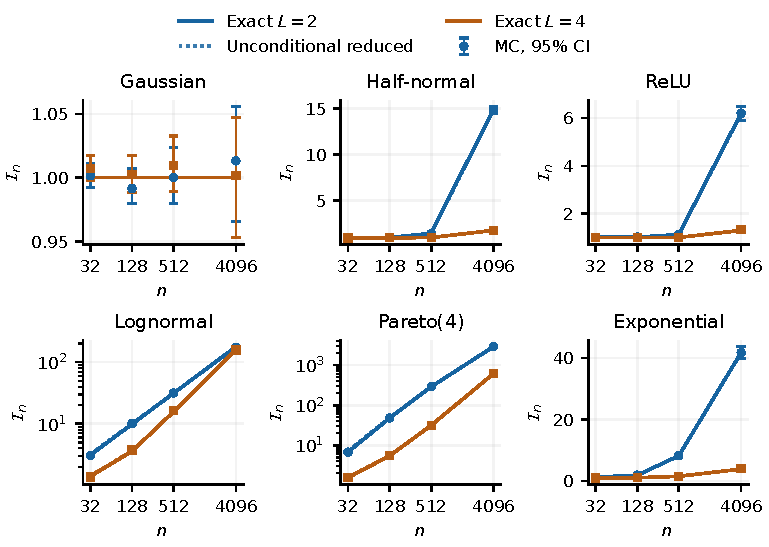
\includegraphics[width=\linewidth]{revision/experiments/figure_benchmark.pdf}
\caption{Finite-block validation on six input laws. Solid curves are exact moment predictions; dotted curves use unconditional responses and drop conditional covariance. Markers show Monte Carlo estimates with 95\% intervals, using conditional stratification for Pareto.}\label{fig:revision-benchmark}
\end{figure}


For asymmetric laws at $n=4096$, $L=2$, the predicted inflation is
$6.205$ for ReLU, $14.927$ for half-normal, $177.1$ for lognormal,
$41.794$ for exponential, and $2894.1$ for Pareto$(4)$.
Changing the precision changes which binades place most inputs in the
zero cell, producing distinct block-length trends.
The conditional-mean upper prediction has maximum additive excess
$0.00648$ in the continuous-law grid. The unconditioned-response
approximation instead has maximum relative discrepancy $5.81\%$,
at Pareto$(4)$, $n=32$, $L=2$: exact inflation is $6.806$, the
conditional-mean upper value is $6.812$, and the unconditioned-response
value is $7.201$. The dominant approximation error here is in the
conditional marginal moments.

Pareto inputs expose the importance of rare scale states. Ordinary
sampling differs from the population prediction by as much as $14.8\%$;
sampling every retained exponent stratum brings all eight predictions
within their intervals. The omitted marginal second-moment bound is
$3.0\times10^{-8}$ at $L=2$ and $1.9\times10^{-9}$ at $L=4$.
Both sampling records are retained.

\paragraph{Rounding controls.}
All eight stochastic-rounding inflation intervals contain one.
At $n=128$, $L=2$, the Gaussian marginal-variance ratio
$12\widehat v/\widehat{\mathbb E[s^2]}$ is approximately $1.000$
for round-to-nearest and $2.000$ for stochastic rounding.
For ReLU, the atom at zero contributes zero error; the ratios are
approximately $1/2$ and $1$, respectively.
These controls check the symmetric residual, conditional unbiasedness,
and treatment of atoms.

\subsection{Weighted reductions and block partition}
For $n=128$, $L=2$, we use positive weights, alternating $1,-1$,
and alternating $1,-0.9$. Define
\begin{equation}\label{eq:weight-imbalance}
 \chi=\frac{(\mathbf1^Tw)^2}{n\|w\|_2^2}\in[0,1].
\end{equation}
Equation~\eqref{eq:revision-weighted} gives
$\mathbb E[E_w^2]/\|w\|_2^2=(v-\kappa)+n(\kappa+\mu^2)\chi$.
The three vectors have $\chi=1$, $0$, and approximately $0.00276$.
Figure~\ref{fig:revision-weighted} and Table~\ref{tab:revision-weighted}
compare shared-scale rounding, split blocks, and independently selected
scales. The predictions have maximum MSE discrepancy $1.48\%$; eleven
of twelve nominal intervals contain them.

% Generated from experiments/tables.tex
\begin{table}[t]
\centering\footnotesize
\caption{Weighted dot-product quantization MSE divided by $\sum_iw_i^2$, lognormal inputs, $n=128$, $L=2$, 50,000 blocks. Brackets are 95\% intervals. The weights are fixed before sampling. Balanced: alternating $1,-1$; near cancellation: alternating $1,-0.9$; positive: all ones.}\label{tab:revision-weighted}
\begin{tabular}{@{}lrrr@{}}\toprule
Method & Balanced & Near cancellation & Positive\\\midrule
Shared RNE & 0.509 [0.500, 0.517] & 0.545 [0.535, 0.555] & 12.58 [12.40, 12.80]\\
Split blocks of 16 & 0.165 [0.162, 0.167] & 0.166 [0.164, 0.168] & 0.816 [0.805, 0.827]\\
Independent scales & 0.020 [0.020, 0.021] & 0.020 [0.020, 0.021] & 0.023 [0.023, 0.024]\\
Shared SR & 1.375 [1.345, 1.407] & 1.374 [1.348, 1.404] & 1.380 [1.350, 1.413]\\
\bottomrule\end{tabular}
\end{table}

% Generated from experiments/figures.tex
\begin{figure}[t]
\centering
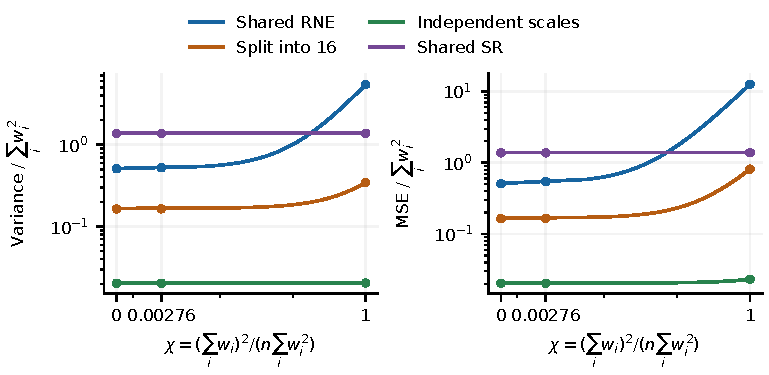
\includegraphics[width=\linewidth]{revision/experiments/figure_weighted.pdf}
\caption{Weighted dot products for lognormal inputs ($n=128$, $L=2$). Fixed weights vary the normalized imbalance $\chi=(\sum_iw_i)^2/(n\sum_iw_i^2)\in[0,1]$. Curves evaluate the affine laws from exact moments on a dense grid; markers show Monte Carlo with 95\% intervals.}\label{fig:revision-weighted}
\end{figure}


Shared round-to-nearest gives normalized MSE $12.58$ for positive
weights and $0.509$ for balanced weights. For positive weights,
centered variance is about $695.1$ and MSE is $1610.0$, showing the
additional squared-bias contribution. Stochastic rounding gives
normalized MSE near $1.38$ for both patterns: eliminating bias and
covariance improves the positive reduction, while its larger marginal
variance worsens the balanced reduction.
Splitting into length-$16$ blocks gives positive-weight MSE $0.816$;
an independent scale per coordinate gives $0.023$. The following
elliptic experiments account for the storage cost of those scale choices.

\paragraph{Asymptotic verification.}
Table~\ref{tab:revision-exponential} evaluates the subsequence in
Theorem~\ref{thm:revision-exponential} at $L=2$, $j=3,\ldots,8$.
Cell integration at $100$ and $160$ digits and the closed exponential
formula agree in all displayed digits. Inflation grows from about $41$
to $4.558\times10^{99}$, while the final $\mathcal I_n/n$ is
$3.016\times10^{-12}$ and the ratio to the theorem normalization is
$0.99999955$.
Here $\mathcal I_n$ is a centered variance ratio; it is not the absolute
mean-square error, whose additional coherent-bias term is given in
\eqref{eq:revision-weighted}. The high-precision calculation resolves
population-moment cancellation and does not claim that a binary64 reduction
would form the displayed sum without overflow or loss of significance.
% Generated from experiments/tables.tex
\begin{table}[t]
\centering\footnotesize
\caption{Exact high-precision exponential counterexample at $L=2$, $n=\lfloor e^{2^j}\rfloor$. The theorem normalization is $C(\log n)^2 n^{7/8}$ with $C=e^{-1}(1-e^{-1})/64$. Convergence of the ratio to one is predicted by the asymptotic theorem. All displayed values agree between 100 and 160 decimal digits.}\label{tab:revision-exponential}
\begin{tabular}{@{}rrrr@{}}\toprule
$2^j$ & $\mathcal I_n$ & $\mathcal I_n/n$ & Exact / normalization\\\midrule
8 & $4.111\times10^{1}$ & $1.380\times10^{-2}$ & 0.161276\\
16 & $3.296\times10^{5}$ & $3.709\times10^{-2}$ & 0.294655\\
32 & $3.298\times10^{12}$ & $4.177\times10^{-2}$ & 0.612870\\
64 & $2.901\times10^{25}$ & $4.652\times10^{-3}$ & 0.931787\\
128 & $2.601\times10^{50}$ & $6.690\times10^{-6}$ & 0.998663\\
256 & $4.558\times10^{99}$ & $3.016\times10^{-12}$ & 1.000000\\
\bottomrule\end{tabular}
\end{table}


\subsection{Spatially heterogeneous sources in an elliptic solve}
\label{sec:revision-elliptic2d}
Consider $-\Delta u=f$ on $(0,1)^2$ with homogeneous Dirichlet conditions.
On an $m\times m$ interior grid, let $h=(m+1)^{-1}$,
$A=h^{-2}(I\otimes T+T\otimes I)$ with
$T=\operatorname{tridiag}(-1,2,-1)$, and $G=A^{-1}$.
We compress the cell sources $b_i=s_i\exp(Z_i)$, where the $Z_i$ are
independent $N(0,1)$ variables. The prescribed spatial scales are
\begin{align*}
 s_{\rm sm}(x,y)&=1+3\sin^2(\pi x)\sin^2(\pi y),\\
 s_{\rm hot}(x,y)&=1+7\exp\!\left(-\frac{(x-0.3)^2+(y-0.65)^2}{0.02}\right).
\end{align*}
These profiles test the nonidentical-input formula with smooth variation
and a localized source hotspot.

Write $e=Q(b)-b$, $\delta u=Ge$, $\mu=\mathbb E e$, and
$\Sigma_B=\operatorname{Cov}(e_B)$ for a partition into disjoint blocks.
For any symmetric positive definite $A$, define $\|z\|_{A,h}^2=h^2z^TAz$.
Independence across blocks gives
\begin{equation}\label{eq:revision-elliptic2d-energy}
 J:=\mathbb E\|\delta u\|_{A,h}^2
 =h^2\left[\sum_B\operatorname{tr}(G_{BB}\Sigma_B)
                 +\mu^TG\mu\right].
\end{equation}
The bias term couples different spatial blocks. Relative RMS is
$\sqrt{J/\{h^2\mathbb E[b^TGb]\}}$, with the denominator evaluated
from the source laws. The baseline denoted Ind. retains every exact
marginal mean and variance while dropping off-diagonal error covariances;
Unif. uses independent zero-mean uniform-cell errors.

All codecs pack exactly $7m^2$ payload bits: an 8-bit signed exponent per
block, $L_B+3$ signed bits per coefficient, and any remaining padding.
Block lengths are $8,32,128$, with contiguous and interleaved layouts.
The largest common precision is supplemented by prescribed extra-bit
blocks. Their locations are fixed codec maps, so no data-dependent flags
are needed. At $m=32$, we compare evenly spaced locations (Uniform),
descending $\sum_{i\in B}s_i^2$ (Source), and a greedy full-energy rule
(Energy). For a candidate precision increment, embed its mean change
$d$ in the full vector and let $\Delta\Sigma_B$ be its block covariance
change. The greedy rule chooses the smallest
\begin{equation}\label{eq:revision-elliptic2d-increment}
 \Delta J=h^2\left[\operatorname{tr}(G_{BB}\Delta\Sigma_B)
                     +2d^TG\mu+d^TGd\right].
\end{equation}
Ties are resolved by block index. The implemented codec rejects
out-of-range exponents; none occurred, and the per-vector probability
bound is below $10^{-1632}$.

We retain all $40$ prescribed configurations, including coincident
precision maps, and use $20\,000$ paired source vectors per profile for
$m=16$ and $60\,000$ for $m=32$, with $300$ whole-vector bootstrap
replicates. The latter pools the initial $10\,000$ vectors and a declared
independent $50\,000$-vector replication for both profiles. All streams,
configuration records, and interval misses remain in the package.
The primary nominal intervals contain 34 of $40$ population RMS predictions;
the largest RMS discrepancy is 0.83\%.

\begin{table}[tb]
\centering
\caption{Two-dimensional heterogeneous source compression, $32^2$ unknowns,
contiguous blocks, and exactly $7168$ payload bits. Source and Energy allocate
the extra coefficient bits by source scale and the full energy prediction,
respectively. Relative energy RMS values are percentages. Ind. retains exact
marginal moments and bias; Unif. uses independent uniform-cell noise.}
\label{tab:revision-elliptic2d}
\begingroup\footnotesize\setlength{\tabcolsep}{3pt}
\begin{tabular}{lrlrrrr}
\toprule
Profile & $|B|$ & Placement & Exact & Ind. & Unif. & MC $95\%$ interval\\
\midrule
Smooth & 8 & Uniform & 1.244 & 1.206 & 1.141 & [1.242,1.248] \\
Smooth & 32 & Uniform & 1.450 & 1.363 & 1.252 & [1.447,1.457] \\
Smooth & 32 & Source & 1.125 & 1.079 & 1.023 & [1.124,1.132] \\
Smooth & 32 & Energy & 1.125 & 1.079 & 1.023 & [1.124,1.131] \\
Smooth & 128 & Uniform & 3.071 & 2.541 & 1.962 & [3.058,3.108] \\
Smooth & 128 & Energy & 2.132 & 1.820 & 1.557 & [2.124,2.159] \\
Hotspot & 8 & Uniform & 1.471 & 1.423 & 1.358 & [1.468,1.481] \\
Hotspot & 32 & Uniform & 1.997 & 1.866 & 1.583 & [2.000,2.016] \\
Hotspot & 32 & Source & 1.543 & 1.451 & 1.282 & [1.544,1.556] \\
Hotspot & 32 & Energy & 1.529 & 1.439 & 1.278 & [1.530,1.542] \\
Hotspot & 128 & Uniform & 4.184 & 3.563 & 2.361 & [4.182,4.233] \\
Hotspot & 128 & Energy & 3.216 & 2.726 & 2.012 & [3.224,3.262] \\
\bottomrule
\end{tabular}\endgroup
\end{table}


For the smooth profile at $m=32$, length-$32$ Energy placement reduces
measured RMS by 22.37\% relative to Uniform placement
(paired $95\%$ interval $[22.17,22.61]\%$).
For the hotspot, it improves on Source placement by 0.86\%
($[0.81,0.91]\%$). These are gains from the full-model
placement objective. The uniform-cell model selects length $32$ with
Energy placement for the hotspot, whereas the exact and marginal-moment
models select length $8$. The former choice has 4.12\% higher
measured RMS ($[3.71,4.48]\%$), so the population model
also supports a concrete accuracy decision at the same storage budget.
The largest covariance gap occurs for the $16^2$ smooth case with
length-$128$ contiguous blocks: exact, Ind., and measured RMS are
5.845\%, 4.769\%, and 5.856\%, respectively;
the diagonal-moment model underestimates energy MSE by a factor 1.50.

For each codec, $100$ paired original and compressed sources are also
solved by conjugate gradients at relative tolerance $10^{-11}$.
For $r=A\widehat{\delta u}-e$, the solver discrepancy satisfies
$\|\widehat{\delta u}-\delta u\|_{A,h}\le h\|r\|_2/
\sqrt{\lambda_{\min}(A)}$; its maximum relative certificate is
$2.8\times10^{-9}$, and the CG and spectral energy values differ by
at most $1.3\times10^{-10}$ relatively.

\subsection{A correlated source field}\label{sec:revision-latent}
For correlated inputs on the $16\times16$ grid, use the same hotspot
envelope $a_i$ and let
\[
 b_i=a_i\exp(Z_i+0.6\phi_iY),\qquad
 \phi_i=\sin(\pi x_i)\sin(\pi y_i),
\]
where $Y,Z_1,\ldots,Z_N$ are independent standard normals.
Corollary~\ref{cor:conditional-mixture} gives the energy prediction
\begin{equation}\label{eq:revision-latent-energy}
 \mathbb E\|\widehat u-u\|_{A,h}^2
 =h^2\mathbb E_Y\!\left[\operatorname{tr}(G\Sigma(Y))
                         +m(Y)^TGm(Y)\right].
\end{equation}
The diagonal comparison replaces $\Sigma(Y)$ by its diagonal while retaining
the entire second term, including the correlations induced by the latent
factor across distinct blocks. The reference source energy is analytical:
for $M_i=a_i\exp((1+0.36\phi_i^2)/2)$,
$\mathbb E[b_ib_j]=M_iM_j\exp(0.36\phi_i\phi_j)$ for $i\ne j$, and
$\mathbb E[b_i^2]=a_i^2\exp(2(1+0.36\phi_i^2))$.

All six prescribed block/layout codecs use $7N$ bits. Gauss--Hermite orders
21, 41, 61 give a final relative change of $2.5\times10^{-13}$ in energy MSE and the
conditional-mean contribution. A new stream of 30\,000 source vectors is paired
across codecs, with 300 vector-bootstrap replicates. The measured
nominal intervals contain all 6 population predictions. Actual CG solves
on 100 vectors per codec have maximum relative energy difference
$8.2\times10^{-11}$ from the direct source-error energies.

\begin{table}[tb]
\centering
\caption{Correlated hotspot sources: relative energy RMS (percent).}
\label{tab:revision-latent}
\begingroup\footnotesize\setlength{\tabcolsep}{4pt}
\begin{tabular}{rlrrl}
\toprule
$|B_j|$ & Layout & Full & Diagonal & MC $95\%$ interval\\
\midrule
8 & Cont. & 2.406 & 2.335 & [2.370,2.428] \\
8 & Inter. & 2.484 & 2.428 & [2.458,2.509] \\
32 & Cont. & 3.124 & 2.832 & [3.068,3.154] \\
32 & Inter. & 3.072 & 2.867 & [3.048,3.119] \\
128 & Cont. & 9.536 & 7.940 & [9.385,9.721] \\
128 & Inter. & 8.171 & 6.989 & [8.002,8.218] \\
\bottomrule
\end{tabular}\endgroup
\end{table}
The diagonal model underestimates energy MSE by as much as a factor
1.44. This comparison isolates the shared-exponent contribution after
the latent source correlation is included; ``diagonal'' here removes only
conditional block off-diagonals and is not a fully independent-source model.

\paragraph{Sensitivity to the common source factor.}
For two fixed contiguous codecs ($|B|=32,128$), we also prescribe
$\tau\in\{0,0.3,0.6,0.9\}$ in $b_i=a_i\exp(Z_i+\tau\phi_iY)$.
Each setting uses $200\,000$ iid source vectors,
paired across codecs, and $1000$ whole-vector bootstrap replicates.
Gauss--Hermite orders $41$ and $61$ differ by at most $9.3\times10^{-9}$ in the
full and comparison energy predictions. The nominal intervals contain
8 of eight population predictions, with maximum RMS discrepancy
0.41\%. This is an empirical interval check rather than a repeated-sampling
coverage claim; all cases are retained in the saved records.
Figure~\ref{fig:latent-sensitivity} shows that removing
conditional block covariances still underestimates MSE throughout this
range. For length $128$, the full/conditional-diagonal ratio changes from
$1.47$ to $1.41$. Removing the latent mean covariances as well increases
the ratio to $1.73$ at $\tau=0.9$. The two losses of covariance are thus
distinct, even in this one-factor family.
\begin{figure}[tb]
\centering
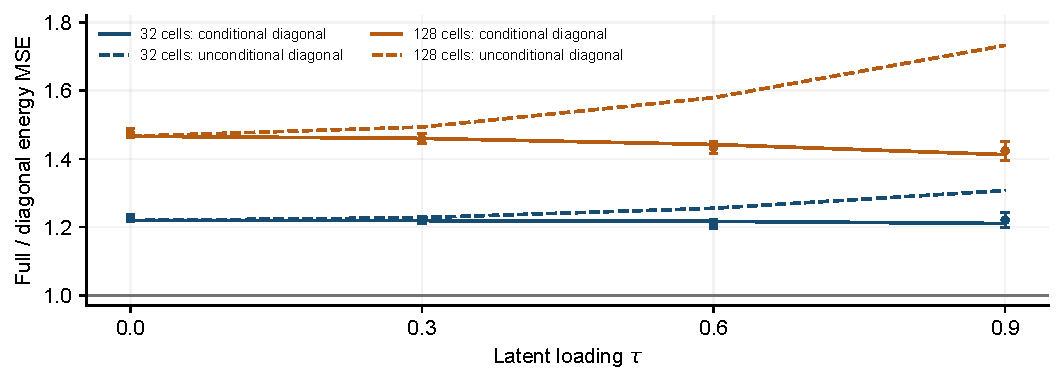
\includegraphics[width=\linewidth]{revision/experiments/latent_correlation_sweep.pdf}
\caption{Common-factor sensitivity at seven bits per source value.
Solid curves retain the full latent mean response in the diagonal comparison;
dashed curves also remove unconditional off-diagonal covariances. Markers
and nominal $95\%$ intervals use independent source vectors.}
\label{fig:latent-sensitivity}
\end{figure}

\subsection{High-contrast diffusion and spatial bit placement}
\label{sec:revision-highcontrast}
We next use $-\nabla\cdot(\alpha\nabla u)=f$ on the same $16^2$ grid,
where $\alpha=0.01$ inside $(x-0.7)^2+(y-0.3)^2\le0.05$ and
$\alpha=1$ elsewhere. Harmonic face conductivities, including the
Dirichlet boundary faces, define the symmetric positive definite operator.
The low-conductivity region is separated from the source hotspot, so the
compression objective accounts for spatial response as well as source scale.
Using the independent hotspot source of Section~\ref{sec:revision-elliptic2d}
and $7$ bits per cell, we retain all
$14$ prescribed codecs and $30\,000$ paired source vectors. At length
$32$, the full-energy rule changes two precision blocks relative to Source
placement: it moves the extra-bit strip from $x\approx0.06,0.12$ toward
the low-conductivity region at $x\approx0.76,0.82$
(Figure~\ref{fig:revision-highcontrast-maps}). This reduces measured RMS by 19.97\%
(paired $95\%$ interval $[19.57,20.37]\%$); at length $128$,
the reduction is 11.25\% ($[10.34,12.17]\%$).
Table~\ref{tab:revision-highcontrast} gives the contiguous results;
both layouts and coincident maps remain in the package. The nominal intervals
contain 13 of $14$ population RMS predictions, with maximum
discrepancy 0.51\%. We also solve $100$ paired sources per codec
by Jacobi-preconditioned conjugate gradients at tolerance $10^{-11}$.
Since $A\succeq0.01A_{\rm Poisson}$, the preceding residual certificate
uses $0.01\lambda_{\min}(A_{\rm Poisson})$; its largest relative bound is
$8.4\times10^{-9}$, while PCG and direct-solve energy values agree within
$4.7\times10^{-11}$ relatively.

\begin{figure}[tb]
\centering
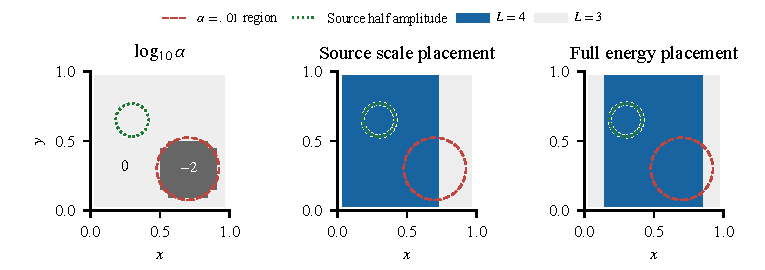
\includegraphics[width=\textwidth]{revision/experiments/highcontrast_precision_maps.pdf}
\caption{The prescribed diffusion coefficient and two length-$32$ contiguous
precision maps. The red disk marks the low-conductivity region; the green
outline is the half-amplitude source contour. Both maps have six blue
$L=4$ blocks and two gray $L=3$ blocks at the same storage cost.}
\label{fig:revision-highcontrast-maps}
\end{figure}

\begin{table}[tb]
\centering
\caption{High-contrast diffusion, $16^2$ sources and exactly $1792$ payload
bits. All entries use contiguous blocks; relative energy RMS is in percent.}
\label{tab:revision-highcontrast}
\begingroup\footnotesize\setlength{\tabcolsep}{5pt}
\begin{tabular}{rlrrr}
\toprule
$|B|$ & Placement & Exact & Ind. & MC $95\%$ interval\\
\midrule
8 & Uniform & 3.213 & 3.159 & [3.202,3.243] \\
32 & Uniform & 4.060 & 3.845 & [4.039,4.103] \\
32 & Source & 3.887 & 3.735 & [3.870,3.925] \\
32 & Energy & 3.114 & 3.005 & [3.099,3.139] \\
128 & Source & 8.948 & 7.993 & [8.817,8.991] \\
128 & Energy & 7.916 & 6.761 & [7.824,7.978] \\
\bottomrule
\end{tabular}\endgroup
\end{table}

\subsection{Calibration from a separate source sample}
\label{sec:revision-calibration}
The preceding high-contrast experiment assumes the source law is known. We
now separate law fitting from codec validation on the same fixed $16^2$
operator. For each $T\in\{32,128,512,2048\}$ and five independently labeled
training samples, we fit $\log b_i=\ell_i+\sigma Z_i$ by coordinate-wise
means and one pooled residual scale. The fitted $(\ell_i,\sigma)$ determine
the source-scale and full-energy bit maps; each map is frozen before a common
30,000-vector validation stream is generated. The uniform map, the oracle
map obtained from the known law, and every learned map are retained; the
validation stream is never used to choose a map.

\begin{table}[tb]
\centering
\caption{Validation RMS and regret for the learned $32$-cell contiguous
maps. Values are medians over five training replicates; regret is relative
to the fixed oracle full-energy map, in percent.}
\label{tab:revision-calibration}
\begin{tabular}{rllrr}
\toprule
$T$ & Source RMS & Energy RMS & Source regret & Energy regret\\
\midrule
32 & 4.498 & 3.100 & 45.07 & 0.00 \\
128 & 3.956 & 3.100 & 27.58 & 0.00 \\
512 & 3.956 & 3.100 & 27.58 & 0.00 \\
2048 & 3.890 & 3.100 & 25.46 & 0.00 \\
\bottomrule
\end{tabular}
\end{table}

The full-moment energy map has median regret 0.00\% at $T=2048$
and 0.00\% at $T=32$; its central 95\% replicate quantile range at $T=32$ is
$[0.00,1.38]\%$. The fitted source scale converges with
$T$ (median log-scale RMSE 0.1714 at $T=32$ versus 0.0222 at
$T=2048$). The median validation error of the train-only full-moment
prediction is -5.43\% at $T=32$ and -1.01\% at $T=2048$.
The fitted energy map recovered the oracle map in 17 of the
20 training fits; the other maps and their validation outcomes are retained.
The validation stream evaluates six unique maps (43 candidate records,
including repeated maps), and all $20$ fits, $40$ learned maps, predictions,
validation energies, and bootstrap intervals are retained. The nominal
intervals contain all six unique-map predictions; repeated candidate rows
are bookkeeping records rather than independent validation tests. The
validation stream is independent of every earlier experiment.


\section{Implications for reductions and compression}\label{sec:discussion}
The moment formulas connect the input distribution, block partition, and
linear operator to the output error. For identical coordinate laws, the
weight sum determines how strongly the common error component enters a
reduction. Balanced weights remove the bias and the term proportional to
$(\mathbf1^Tw)^2$, leaving $(v-\kappa)\|w\|_2^2$. Positive weights can
instead accumulate both covariance and bias. This explains why stochastic
rounding can improve a positive-weight reduction while increasing the
mean-square error of a balanced one: its larger marginal variance is then
the deciding term. The appropriate rounding rule depends on the weights
and the accuracy criterion.

Partitioning changes both the selected scales and the covariance structure.
Each candidate partition therefore requires its own moments. The storage
cost of additional scales also changes the available coefficient precision.
In an elliptic solve, block layout further determines how the covariance
aligns with the Green operator. A model that retains only marginal error
variances loses this interaction, even when it estimates those variances
accurately. The equal-budget experiments demonstrate how the complete
moments predict solution error and guide the comparison of prescribed
compression choices. The calibration experiment shows how this workflow
degrades when the source law is estimated from a separate sample.

Block length and total problem size have different effects. If $N=Kn$
independent inputs occupy $K$ identical blocks of fixed length $n$, their
total error satisfies
\begin{equation}\label{eq:multiblock-mse}
 \mathbb E\left[\left(\sum_{i=1}^{N}e_i\right)^2\right]
 =Nv\mathcal I_n+N^2\mu^2.
\end{equation}
The centered standard deviation grows as $\sqrt N$, while a nonzero mean
error contributes quadratically to mean-square error. An inflation factor
describes the centered component; accuracy assessment requires both terms.

The exponential counterexample concerns growth of the block itself. At
fixed grid precision, its increasing maximum makes each fixed coordinate
eventually round to zero. The error approaches the negative input, and
pair correlation vanishes, but multiplication by $n-1$ still permits
diverging inflation. The dyadic location of the maximum produces pronounced
changes with block length. The exact finite-block evaluator resolves these
changes without extrapolating a power law from one phase.

Latent factors separate a structured field's common fluctuations from its
independent innovations. Conditional moment evaluation preserves dependence
between spatial blocks through the varying mean error. More general joint
laws require joint truncated moments; data-dependent weights require mixed moments of
the weights and quantization errors. Quantizing both operands and including
product or accumulation rounding adds further error terms. Saturation,
nonuniform element grids, and finite random bits can be incorporated by
supplying the corresponding scalar quantizer moments
\cite{elarar2024}.
The applications use a uniform integer-mantissa grid with an 8-bit signed
exponent and binary64 arithmetic. They establish accuracy comparisons at a
fixed payload budget for specified source laws and discrete operators.
Transfer to measured scientific fields, nonuniform MX element grids,
saturation, and low-precision accumulation requires separate validation.
Encoding cost, memory traffic, and solver speed were not measured.

\section{Conclusions}\label{sec:conclusions}
Maximum-selected block quantization creates two competing covariance terms:
variation of the conditional error mean and the correction caused by
excluding an all-small block. One-dimensional truncated moments compute
both exactly and give variance and mean-square error predictions for
weighted reductions. For identical input laws, dropping the conditional
pair correction has a distribution-free additive error bound of one in
the variance inflation factor. The heterogeneous and conditional-mixture
extensions supply the covariance for spatially varying and correlated sources.

The support limits and exponential counterexample show why fixed-pair
decorrelation does not imply unit inflation. The experiments verify the
finite-block identities and connect the resulting moments to weight
balance, storage allocation, spatial layout, and elliptic solution error.
Together, the analysis and evaluator turn a statistical quantization model
into a computable accuracy prediction for a specified input law and
compression design.

\section*{Data and code availability}
The accompanying reproduction package contains the experiment driver, saved
machine-readable results, figure and table generator, high-precision evaluator,
exact rational enumeration oracle, and a manifest with random seeds, package
versions, execution times, and file hashes. The figures and tables in this
manuscript are generated from that package. The existing project repository is
\url{https://github.com/NUAApanda-1116/bfp-error-independence}; it records the
project history, while the accompanying revision package is the submitted
snapshot and specifies the files required to reproduce this version.
\bibliographystyle{siamplain}
\bibliography{references}
\end{document}

